\chapter{Related Work} \label{Related Work}

Due to the specific characteristics of both the problem that we wish to solve and the models in which we propose to solve it, there are several areas that contain works of interest to us. Section \ref{Paxos} describes previous work regarding consensus and several Paxos variants. Section \ref{Non-Crash} discusses non-crash fault models as well as protocols that solve consensus in these environments. Section \ref{Partial Synchrony} describes different partial synchrony models and how they fit in the synchrony spectrum. Section \ref{Variable Consistency} discusses variable consistency models that attempt to strike a balance between strong and weak consistency in order to obtain advantages from both. Despite the fact that the Paxos protocol family has been a subject of study for some time, this topic is now more relevant than ever since these algorithms have become widely used by the industry to implement large-scale, highly available services \cite{Burrows2006,Hunt2010}. Section \ref{Coordination Systems} studies a few systems where these algorithms are used to enable fault-tolerance services.

\section{Paxos and its Variants} \label{Paxos} 
\textbf{Classic Paxos.} The Paxos protocol family solves consensus by circumventing the well-known \acrshort{flp} impossibility result \cite{Fischer1985}. It does this by making the observation that, while consensus is unsolvable in asynchronous systems, most of the time systems can be considered synchronous since delays are sporadic and temporary. Therefore, as long as consistency is guaranteed regardless of synchrony, Paxos can forgo progress during the temporary periods of asynchrony. Using this insight, Paxos ensures consistency even when the system is asynchronous but can only guarantee progress while it is synchronous and no more than $f$ faults occur for a system of $2f+1$ replicas \cite{Lamport2001}. The classic form of Paxos employs a set of proposers, acceptors and learners and runs in a sequence of ballots. To ensure progress during synchronous periods, proposals are serialized by a distinguished proposer, the leader. It is the leader that gathers proposals from other proposers and requests, in a \textit{phase 1a} message, that acceptors promise to not accept any ballots smaller than its own. Each acceptor responds to the leader's request, in a \textit{phase 1b} message, with either a promise or a message stating that it has already sent a promise to a proposer with a higher-numbered ballot. If the leader manages to obtain a promise from a quorum of acceptors, then it sends a \textit{phase 2a} message containing its proposal. The acceptors may accept the proposal and inform the learners with a \textit{phase 2b} message, if another proposer hasn't requested a promise for a higher-numbered ballot in the meanwhile. The fact that any proposer can request a promise and prevent lower ballots from being completed is the reason why Paxos can only ensure progress when an environment is in a synchronous period. Some proposer must be able to establish itself as the only leader in order to prevent proposers from continuously requesting promises for ballots with higher numbers. \par
\textbf{Multi-Paxos.} We now describe the form in which Paxos is most commonly deployed, Multi(Decree)-Paxos. Multi-Paxos provides an optimization of the basic Paxos' message pattern by omitting the first phase of messages from all but the first ballot for each leader \cite{Renesse2011}. This means that a leader only needs to send a \textit{phase 1a} message once and subsequent proposals may be sent directly in \textit{phase 2a} messages without requesting a promise from the acceptors. This reduces the message pattern in the common case from five message delays to just three (from proposal to learning). Since there are no implications on the quorum size or guarantees provided by Paxos, the reduced latency comes at no additional cost. \par
\textbf{Fast Paxos.} Fast Paxos observes that it's possible to improve on previous results by allowing proposers to propose values directly to acceptors~\cite{Lamport2006}. To this end, the protocol distinguishes between fast and classic ballots, where fast ballots bypass the leader by sending proposals directly to acceptors and classic ballots work as in the original Paxos protocol. 
\begin{figure}
	\centering
	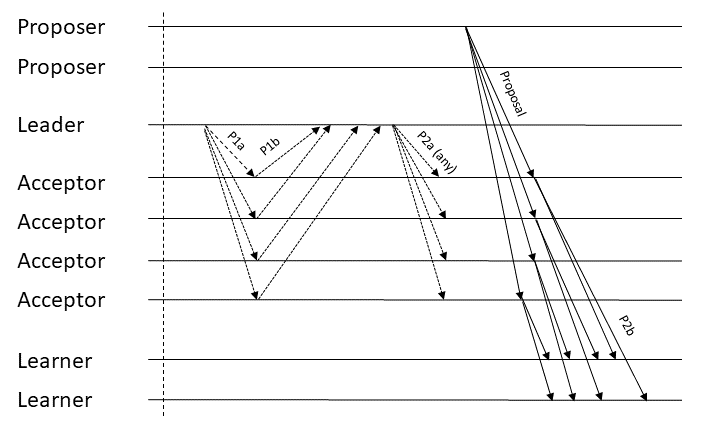
\includegraphics[width=\textwidth*2/3]{Figures/fast_paxos}
	\caption{Fast Paxos' fast ballot message pattern}
	\label{fast_paxos_fig}
\end{figure}
The fast ballots' reduced latency comes at the additional cost of using a quorum size of $N-e$ instead of a classic majority quorum, where $e$ is the number of faults that can be tolerated while using fast ballots. In addition to the usual requirement that $N> 2f$, to ensure that fast and classic quorums intersect, a new requirement must be met: $N > 2e+f$. This means that if we wish to tolerate the same number of faults for classic and fast ballots (i.e., $e=f$), then the total number of replicas is $3f+1$ instead of the usual $2f+1$ and the quorum size for fast and classic ballots is the same. However, we can also choose to maximize $f$ instead of $e$ and the classic quorum becomes a majority quorum while a fast quorum must be larger than $\lceil \frac{3N}{4} \rceil$. This configuration is interesting since we can tolerate the largest possible number of faults but fast ballots are only possible if a larger number of replicas are correct. The optimized commit scenario occurs during fast ballots, in which only two message broadcasts are necessary: \textit{proposal} messages between a proposer and the acceptors, and \textit{phase 2b} messages between acceptors and learners. This is shown in Figure~\ref{fast_paxos_fig}, where dotted lines represent messages that only need to be exchanged once per ballot and solid lines represent messages that can be exchanged more than once. This message pattern creates the possibility of two proposers concurrently proposing values to the acceptors and generating a conflict. The cost of dealing with this conflict depends on the chosen method of recovery, coordinated or uncoordinated, and if the leader or acceptors are also learners. The leader may choose  the recovery method in the beginning of the ballot. If coordinated recovery is chosen in a ballot $i$, then the acceptors send \textit{phase 2b} messages both to the learners and to the leader, who performs the conflict detection. After a conflict is detected, the leader picks a value and sends it in a \textit{phase 2a} message to the acceptors. The cost of recovery with this method is equivalent to a \textit{phase 2} of round $i+1$ (i.e., two additional message delays). If uncoordinated recovery is chosen, the acceptors also broadcast \textit{phase 2b} messages between each other and, if necessary, pick a value is some deterministic way and send it in a \textit{phase 2b} message to the learners. The cost of this approach is a single message in round $i+1$ (i.e., one message delay) but more messages have to be exchanged than in coordinated recovery. \par
\textbf{Generalized Paxos.} Generalized Paxos addresses Fast Paxos' shortcomings regarding collisions. More precisely, it allows acceptors to accept different sequences of commands as long as non-commutative operations are totally ordered \cite{Lamport2005}.  Non-commutativity between operations is generically represented as an interference relation. Generalized Paxos abstracts the traditional consensus problem of agreeing on a single value to the problem of agreeing on an increasing set of values. \textit{C-structs} provide this abstraction of an increasing set of values and allow us to define different consensus problems. If we define the sequence of learned commands of a learner $l_i$ as a \textit{c-struct} $learned[l_i]$, then the consistency requirement for consensus can be defined as:
\begin{itemize}
\item \textbf{Consistency} -- $learned[l_1]$ and $learned[l_2]$ are always compatible, for all learners $l_1$ and $l_2$.
\end{itemize}
For two \textit{c-structs} to be compatible, they must have a \textit{common upper bound}. This means that, for any two learned \textit{c-structs} such as $learned[l_1]$ and $learned[l_2]$, there must exist some \textit{c-struct} to which they are both prefixes. This prohibits non-commutative commands from being concurrently accepted because no subsequent \textit{c-struct} would extend them both since it wouldn't have a total order of non-commutative operations. For instance, consider a set of commands $\lbrace A$, $B$, $C\rbrace$ and an interference relation between commands $A$ and $B$ (i.e., they are non-commutative with respect to each other). If proposers propose $A$ and $C$ concurrently, some learners may learn one command before the other and the resulting \textit{c-structs} would be either $C \bullet A$ or $A \bullet C$. These are compatible because there are \textit{c-structs} that extend them, namely $A \bullet C \bullet B$ and $C \bullet A \bullet B$. These \textit{c-structs} that extend them are valid because the interfering commands are totally ordered. However, if two proposers propose $A$ and $B$, learners could learn either one in the first ballot and these \textit{c-structs} would not be compatible because no \textit{c-struct} extends them. Any \textit{c-struct} would start either by $A \bullet B$ or $B \bullet A$, which means that an interference relation would be violated. In the Generalized Paxos protocol, when such a collision occurs, no value is chosen and the leader intervenes by starting a new ballot and proposing a \textit{c-struct}. Defining \textit{c-structs} as command histories enables acceptors to agree on different sequences of commands and still preserve consistency as long as dependence relationships are not violated. This means that commutative commands can be ordered differently regarding each other but interfering commands must preserve the same order across each sequence at any learner. This guarantees that solving the consensus problem for histories is enough to implement a state-machine replicated system. \par
\textbf{MDCC.} \acrfull{mdcc} is an optimistic commit protocol that uses Generalized Paxos for transaction processing. \acrshort{mdcc} uses fast commutative ballots to commit several commutative updates in the same ballot with potentially different orders across storage nodes~\cite{Kraska2013}. To preserve global constraints (e.g., the stock should never go below zero), a demarcation technique is used to limit the amount of transactions that can be committed in a ballot. \acrshort{mdcc} is one of the few works that takes advantage of Generalized Paxos to concurrently commit commutative operations.\par
\textbf{Mencius.} Mencius is also a variant of Paxos that tries to address the bottleneck of having a single leader through which every proposal must go through. In Mencius, the leader of each round rotates between every process. The leader of round $i$ is the process $p_k$, such that $k = n\ mod\ i$.  Leaders with nothing to propose can skip their turn by proposing a \textit{no-op}. If a leader is slow or faulty, the other replicas can execute \textit{phase 1} to revoke the leader's right to propose a value but they can only propose a \textit{no-op} instead \cite{Mao2008}. Considering that non-leader replicas can only propose \textit{no-ops}, a \textit{no-op} command from the leader can be accepted in a single message delay since there is no chance of another value being accepted. If some non-leader server revokes the leader's right to propose and suggests a \textit{no-op}, then the leader can still suggest a value $v \neq$ \textit{no-op} that will eventually be accepted as long as $l$ isn't permanently suspected. The usage of an unreliable failure detector is enough to guarantee that eventually all faulty processes, and only those, will be suspected. Mencius also takes advantage of commutativity by allowing out-of-order commits, where values $x$ and $y$ can be learned in different orders by different learners if there isn't a dependence relationship between them. Experimental evaluation confirms that Mencius is able of scaling to a higher throughput than Paxos. \par
\textbf{EPaxos.} \acrfull{epaxos} extends Mencius' goal of achieving a better throughput than Paxos by removing the bottleneck caused by having a leader. Additionally, EPaxos also achieves optimal commit latency in certain conditions and graceful performance degradation if replicas fail or become slow \cite{Moraru2013}. To avoid choosing a leader, the proposal of commands for a command slot is done in a decentralized manner. Each replica can propose a command with ordering constraints attached so that interfering commands can be totally ordered. In this way, \acrshort{epaxos} takes advantage of the commutativity observations made by Generalized Paxos that state that commutative commands may be ordered differently at different replicas without losing state convergence \cite{Lamport2005}. If two replicas unknowingly propose commands concurrently, one will commit its proposal in one round trip after getting replies from a quorum of replicas. However, some replica will see that another command was concurrently proposed and may interfere with the already committed command. If the commands are commutative then there is no need to impose a particular order but, if they're not commutative, then the replica must reply with a dependency between the commands. If a replica commits a command $A$ in a single round trip, then the replica that tries to concurrently propose a non-commutative command $B$ would receive a reply with the ordering $B \rightarrow \{A\}$, to indicate that $B$ should be committed after $A$. In this scenario, committing command $B$ would require two round trips since the proposer would need to send another message to inform the other replicas of the new ordering constraint. This commit latency is achieved by using a \textit{fast-path quorum} of $f+\lfloor\frac{f+1}{2}\rfloor$ replicas which is the same as the \textit{slow-path quorum} of $f+1$ replicas, for $f \leq 2$. Similarly to Mencius, \acrshort{epaxos} achieves a substantially higher throughput than Multi-Paxos, especially when $2\%$ of commands interfere with each other. However, since, unlike Mencius, replicas don't have to wait for previous replicas to propose their commands, commit latency can be significantly lower.\par
\textbf{Raft.} Raft is a consensus protocol that manages a replicated log which is used to implement \acrshort{smr} among replicas~\cite{184040}. This protocol is similar to Paxos in terms of the performance and assurances that it provides but has the additional goal of striving for better understandability. To this end, unlike Paxos, Raft separates leader election, log replication and safety into distinct components. The leader uses a heartbeat mechanism to inform the \textit{followers} that it hasn't crashed. If a follower doesn't receive a message from the leader for a period greater than the \textit{election timeout}, it increments the \textit{term}, begins an election and transitions to the \textit{candidate} state. In this state, the replica votes for itself and requests votes from other processes. A candidate wins the election and becomes the leader if it receives votes from a majority of replicas in the cluster. To ensure that eventually some \textit{candidate} is elected as the leader, election timeouts are randomized to reduce the probability that multiple servers will timeout at the same time and divide the votes. Log replication is performed by having the leader service client requests, which contain commands to be executed by the state machines. The leader appends each command to its log and requests that followers do the same. When the leader sends a new entry to the followers, it also sends the corresponding index and term so that a follower can check if it's missing commands before adding the new one to its log. This consistency check ensures that the logs match during normal operation. However, a leader can fail before fully replicating new entries to the followers, which can cause divergence between the followers' and the new leader's logs. To reintroduce consistency between the two logs, the leader finds the latest entry in which both agree, deletes later entries in the follower's log and sends the entries that it has after that point. However, the restrictions and checks described so far are not enough to guarantee safety, in particular because a follower might not write a leader's entries, then be elected as the leader and overwrite the followers' logs. To prevent this from happening, Raft restricts the candidates that can be elected as the leader by ensuring that the new leader's log contains every committed entry. This is done by including information about the candidate's log when requesting votes. If the voter's log is more up-to-date than the candidate's log, the voter refuses to vote for it. Since the leader must obtain a majority of votes and an entry is only committed after also gathering a majority of votes, the leader is sure to contact at least one process that has committed the latest value. \par
\textbf{Viewstamped Replication.} Viewstamped Replication is a replication technique based on a primary-backup scheme where the system is composed of multiple groups that contain several \textit{cohorts}~\cite{Oki:1988}. In each group, one cohort is the primary and the remaining are the backups. If the primary crashes, a view-change protocol is executed and one of the backup replicas becomes the new primary. The system makes progress by having client groups create transactions composed of several procedure calls and making those calls to server groups. When a transaction terminates, a two-phase commit protocol is executed to replicate the corresponding changes. The client's primary acts as the coordinator for the commit protocol and the servers' primaries act as participants. Events such as the processing of procedure calls or prepare messages are written to the communication buffer as records (and possibly flushed to the backups), to ensure that the committed transactions are not lost. Viewstamped Replication also introduces \textit{viewstamps} which are the concatenation of \textit{timestamps}, which are unique within a view, and \textit{view identifiers}. Each replica in the system maintains viewstamps in a sequence, the \textit{history}, for each event that is reflected in its state. These viewstamps are used to determine if, after the failure of a primary, the effects of an on-going transaction survived and it can commit or if it must be aborted. \par
Even though some Paxos variants attempt to improve on the original protocols by removing the bottleneck caused by having a single leader or by shortening the number of message steps in the common case, few works align these improvements with non-crash fault models. Our \acrlong{bgp} protocol attempts to bridge the gap between these two types of extensions to consensus-solving protocols in order to make their usage more viable within datacenters where arbitrary faults occur.

\section{Protocols for Non-Crash Fault Models} \label{Non-Crash}
Non-crash fault models emerged to cope with the effect of malicious attacks and software errors. These models (e.g., the arbitrary fault model) assume a stronger adversary than previous crash fault models. The Byzantine Generals Problem is defined as a set of Byzantine generals that are camped in the outskirts of an enemy city and have to coordinate an attack. Each general can either decide to attack or retreat and there may be $f$ traitors among the generals that try to prevent the loyal generals from agreeing on the same action. The problem is solved if every loyal general agrees on what action to take \cite{Lamport1982}. Like the traitorous generals, the Byzantine adversary is one that may force a faulty replica to display arbitrary behaviour and even coordinate multiple faulty replicas in an attack. It's interesting to survey non-crash fault models since we intend to explore the effects that different models have on the solutions for the generalized consensus problem. \par
\textbf{PBFT.} \acrfull{pbft} is a protocol that solves consensus for \acrshort{smr} while tolerating up to $f$ Byzantine faults \cite{Castro1999}. The system moves through configurations called \textit{views} in which one replica is the primary and the remaining replicas are the backups. The safety property of the algorithm requires that operations be totally ordered. The protocol starts when a client sends a request for an operation to the primary, which in turn assigns a sequence number to the request and multicasts a \textit{pre-prepare} message to the backups. This message contains the timestamp, the digest of the client's message, the view and the actual request. If a backup replica accepts the pre-prepare message, after verifying that the view number and timestamp are correct, it multicasts a \textit{prepare} message and adds both messages to its log. The prepare message is similar to the pre-prepare message except that it doesn't contain the client's request message. Both of these phases are needed to ensure that the requested operation is totally ordered at every correct replica. The protocol's safety property requires that the replicated service must satisfy linearizability, and therefore operations must be totally ordered. After receiving $2f$ prepare messages, a replica multicasts a \textit{commit} message and commits the message to its log when it has received $2f$ commit messages from other replicas. The liveness property requires that clients must eventually receive replies to their requests, provided that there are at most $\lfloor\frac{N-1}{3}\rfloor$ faults and the transmission time doesn't increase continuously. This property represents a weak liveness condition but one that is enough to circumvent the \acrshort{flp} impossibility result \cite{Fischer1985}. A Byzantine leader may try to prevent progress by omitting pre-prepare messages when it receives operation requests from clients, but backups can trigger new views after waiting for a certain period of time. \par
Several other \acrfull{bft} protocols have been proposed which extend the initial protocol in different directions, such as the use of trusted components in order to reduce the replication factors~\cite{minbft,kapitza2012}, finding new building blocks to easily construct new Byzantine protocols~\cite{Guerraoui2008}, or weakening the fault model while still supporting arbitrary faults in order to reduce the replication factor and quorum size. From these extensions the ones that are more directly related to this thesis are those that target data center environments and geo-replicated systems, where heightened security makes coordinated Byzantine behavior unlikely but the large amounts of equipment increase the occurrence of arbitrary faults due to hardware failures~\cite{Porto2015,Liu2015}. This is due to our initial motivation of developing protocols that target geo-replicated systems hosted across multiple datacenters, in which not only faults are a common occurrence but there is also a need for reducing hardware and power costs.\par
\textbf{VFT.} The creators of \acrfull{vft} also make the observation that the Byzantine model is too pessimistic, especially for environments such as data centers~\cite{Porto2015}. The Byzantine adversary's strength forces protocols to incur in an unnecessary cost of $3f+1$ replicas. VFT also notes that while data centers rarely observe arbitrary coordinated faults, they commonly experience data corruption faults (e.g., bit flips) and these also represent a type of arbitrary behaviour \cite{AmazonS31,AmazonS32}. To reconcile the need to tolerate different types of arbitrary faults, VFT observes that it is very unlikely for data corruption to affect the same data across multiple replicas. Therefore, the key distinguishing factor between these types of arbitrary faults is \textit{correlation}. \acrshort{vft} proposes a customizable model that defines a limit of $u$ faults, that bounds the number of allowed omission (i.e., crash) and comission (i.e., arbitrary) faults, a limit of $o$ correlated comission faults, a limit of $r$ arbitrary faults and, for every process $p_i$, $s$ correct processes $p_j$ that are slow with respect to it. These additional assumptions allow the Visigoth model to decrease the replication factor from $N \geq 2u+r+1$ (i.e., $3f+1$ in the traditional notation) to $N \geq u+s+o+1$, when $u > s$. These parameters allow the system administrator to configure the system to tolerate any combination of faults. The authors also propose a VFT state machine replication protocol, which is adapted from the BFT-SMaRt protocol~\cite{Bessani:2014} and contains two main message patterns: the first consists in two message steps that are executed during epoch changes to collect information about previous epochs and disseminate this information to replicas; and the second consists in two multicast phases that are executed for each client request to implement the replicated state machine. To gather a quorum, the gatherer tries to collect a larger quorum of $N-s$ replies, which can be seen as collecting replies from the fast but potentially faulty replicas. If a timeout occurs, the quorum is reduced to $N-u$ and this can be seen as collecting replies from correct but possibly slow replicas. This reduced quorum size is enough to ensure an intersection because, since $x$ replicas didn't reply by the first timeout and only $s$ may be slow, $x-s$ replicas must have crashed and won't participate in future quorums. The experimental evaluation confirms that \acrshort{vft} can tolerate uncorrelated arbitrary faults with resource-efficiency and performance that resembles that of \acrshort{cft} systems instead of \acrshort{bft}. \par
\textbf{XFT.} The cost of $3f+1$ replicas in a \acrshort{pbft} system stems from the immense power given to the adversary. The \acrfull{xft} model claims that this adversary is too strong when compared to the behavior of deployed systems~\cite{Liu2015}. XFT assumes that machine and network faults are uncorrelated and this assumption allows it to have a cost equal to crash fault tolerant systems, $2f+1$, while still tolerating $f$ non-crash faults. The safety condition for this model is that correct replicas commit requests in a total order, as long as the system is not in anarchy. A system is in anarchy if there are any non-crash faults $f_{nc}$ and the sum of crash faults $f_c$, non-crash faults $f_{nc}$ and partitioned replicas $f_p$ is larger than the fault threshold. That is, the system is in anarchy at a given moment $s$ if and only if $f_{nc}(s) > 0\ \land\ f_{nc}(s)+ f_c(s)+f_p(s) > f$. Liveness is also guaranteed as long as the system is outside of anarchy. \acrshort{xft} replicates client requests to $f+1$ replicas synchronously while the remaining $f$ may learn about requests through lazy replication \cite{Ladin1992}. If an active replica fails, a view change is triggered. A view change requires all the replicas in the new view to collect the recent state, including the commit log, which may be substantial. This overhead can be decreased through the use of checkpointing. The protocol includes the exchange of four rounds of messages: SUSPECT, VIEW-CHANGE, VC-FINAL and NEW-VIEW. The experimental evaluation performed by the authors shows that, after each crash, the system triggers a view change that last less than 10 seconds (note that this value is dependent on network quality and other details). \par
\textbf{Self-stabilizing Systems.} Dijkstra proposed self-stabilizing systems as a solution to the problem of keeping cyclic sequences of processes (i.e., processes connected to two neighbors, forming a ring) in a legitimate state even after the occurrence of transient faults \cite{Dijkstra1974}. In this self-stabilizing system, each process may contain several privileges and may only exchange information with its neighbors. A privilege is a boolean function on the state of the machine and the state of its neighbors. The requirement of keeping the system in a legitimate state is met if: (1) one or more privileges are present; (2) in each state, the possible moves transfer the system to a legitimate state again (3) each privilege exists in at least one legitimate state; and (4) for any pair of legitimate states, there is a sequence of moves that transfers the system from one to the other. These systems define a set of rules for transferring privileges in a way such that a system that starts from an arbitrary state is guaranteed to converge to a legitimate state and remain in a set of legitimate states. Self-stabilizing systems are an example of a non-crash model that isn't strictly stronger than crash fault models since, due to the system's ring-like structure, a crash fault would render the system unusable. A self-stabilizing system tolerates any arbitrary corruption of the state but, unlike other non-crash models, it assumes that a process always executes correct code.\par
\textbf{ASC.} The \acrfull{asc} model defines ASC faults as faults that occur at a process $p$ and either make it crash or assign an arbitrary value to a variable of the process's state. The assignment of an arbitrary value to a variable of $p$'s state may also alter its control flow in a way such that the process may execute any of its instructions \cite{Correia2012}. This modeling stems from three main observations: (1) most tolerable failures are caused by state corruptions instead of malicious behavior, (2) control-flow faults are very likely to cause incorrect outputs \cite{Kalbarczyk2003}, and (3) the relevant failures are caused by transient faults instead of permanent faults being repeatedly activated. In the context of this model, the ASC hardening technique is proposed to deal with ASC faults. This technique guarantees that, if a correct hardened process $p_c$ receives a message $m$ from a faulty hardened process $p_{f1}$, then $p_c$ discards $m$ without modifying its state. If a faulty process $p_{f2}$ receives $m$ and modifies its local state, then it crashes before sending an output message. ASC hardening uses message integrity checks to prevent network corruption faults and state integrity checks to replicate process state. Every time a value is read from a variable, it's checked against the replicated value. If a mismatch occurs, the process crashes itself to preserve integrity. Control-flow faults are prevented through the use of gates, which are sequences of instructions that ensure that a portion of code is executed the appropriate number of times. For instance, we may want to ensure that an event handler executes exactly once per event. For each control-flow gate, two variables and a label are created, respectively, $c$, $c'$ and $L$. A gate executes a sequence of checks and assignments to ensure the required semantics. A useful type of control-flow gate is an \textit{at-most-once} gate, which ensures that code isn't executed twice even in the presence of faults. An \textit{at-most-once} gate implements these semantics by crashing the process if $c \neq c' \vee c=L$. In the first execution of the code, the condition fails, both $c$ and $c'$ are set to $L$ and the execution continues. In a second execution, the condition would evaluate to true since $c$ has already been set to $L$ and the process would crash. The $c \neq c'$ condition prevents an arbitrary state fault from corrupting the variable's value. Another relevant type of control-flow gate is an \textit{at-least-once} gate, which ensures that a gate has been executed before. For an \textit{at-least-once} gate, if $c=c'=L$ the gate has been reached before. Otherwise, the process crashes itself. ASC is similar to self-stabilizing systems \cite{Dijkstra1974} in the sense that both assume that only state can become corrupted, while the executed code is always correct. An \acrshort{asc}-hardened implementation of Paxos has a throughput up to 70\% higher than \acrshort{pbft}. \par
\textbf{Zeno.} Zeno is a Byzantine fault tolerance \acrshort{smr} protocol that favors availability instead of consistency \cite{Singh2009}. By trading strong consistency for eventual consistency, Zeno provides higher availability when network partitions occur and better performance when replica latency is heterogeneous.  A client request is said to be \textit{weakly complete} if the client gathers matching replies from a \textit{weak quorum} of $f+1$ replicas. This ensures the client that at least one correct replica will execute the request and commit it to the linear history. For a request to be \textit{strongly complete}, the client must wait for matching replies from a \textit{strong quorum} of $2f+1$ replicas. In the case of a partition, two clients concurrently issuing requests may cause divergent histories that can later be merged to restore consistency between replicas. When a replica receives a client request, it performs the appropriate security checks (e.g., message authenticity, correct view, etc) and executes the requested operation. If the request was for a weak operation, the replica replies to the client immediately after the operation terminates. However, if the request was for a strong operation, the replica multicasts a \textit{COMMIT} message to the other replicas and waits for $2f$ matching messages. After receiving $2f$ \textit{COMMIT} messages, the replica forms a commit certificate for the messages it received, stores it and replies to the client. To further increase availability, Zeno's view change protocol is also guaranteed to proceed with only a weak quorum of replicas. Strongly consistent \acrshort{bft} systems require view change protocols to gather a strong quorum to ensure that a view change quorum intersects with any other quorum in at least one correct replica. If this property isn't ensured, another quorum could commit a request that would be unseen by the view change. In Zeno, a request can go unnoticed by view change quorum, resulting in divergent histories and a subsequent merge. \par
\textbf{WHEAT.} \acrfull{wheat} is a \acrshort{wan}-optimized \acrshort{smr} protocol implemented on top of BFT-SMaRt, a \acrshort{bft} consensus protocol with a message pattern similar to \acrshort{pbft}~\cite{Sousa2016,Bessani:2014}. \acrshort{wheat} employs a number of optimizations that were empirically shown to produce the most results in improving the latency of \acrshort{smr} in wide-area networks. The first two optimizations, \textit{read-only} and \textit{tentative executions}, were introduced in \acrshort{pbft} with the goal of reducing the number of communication steps~\cite{Castro1999}. Since read-only operations don't modify the service's state, replicas can execute a request immediately after checking its authenticity and verifying that it is indeed read-only. The reply to the client can be sent after other requests reflected in the tentative state have committed. Tentative executions allow a replica to execute a request tentatively after it has been prepared by a Byzantine quorum, instead of locally committed. This means that the request can be executed after the first all-to-all round instead of the second. However, both optimizations require the client to wait for $2f+1$ replies instead of $f+1$. The authors also determine that it's possible to reduce latency by adding replicas to the system while maintaining the quorum size. However, this isn't possible with traditional quorum gathering due to safety violations. To take advantage of this optimization without sacrificing safety, \acrshort{wheat} uses weighted replication where, instead of requiring a quorum to access a majority of replicas, a quorum must obtain a majority of votes. The optimization is enabled by assigning a higher number of votes to replicas with better connectivity or performance. For instance, in a \acrshort{cft} system of four replicas, three could have a weight of 1 and the fourth could have a weight of 2. To achieve a majority vote, a quorum would have to obtain at least 3 votes, which can be done by gathering votes from three replicas with a weight of 1 or from two replicas, one with a weight of 1 and another one with a weight of 2. The same reasoning applies in \acrshort{bft} mode with the difference that a quorum would have to reach a Byzantine majority of votes. The value of these optimizations is validated by the experimental evaluation which reports a $37\%$ and $58\%$ global median improvement in latency in the \acrshort{bft} and \acrshort{cft} models, respectively. \par
\textbf{FaB Paxos.} Perhaps the most closely related work is \acrfull{fab} Paxos, which solves consensus in the Byzantine setting within two message communication steps in the common case, while requiring $5f+1$ acceptors to ensure safety and liveness \cite{Martin2006}. A variant that is proposed in the same paper is the Parameterized \acrshort{fab} Paxos protocol, which generalizes \acrshort{fab} Paxos by decoupling replication for fault tolerance from replication for performance. As such, the Parameterized \acrshort{fab} Paxos requires $3f+2t+1$ replicas to solve consensus, preserving safety while tolerating up to $f$ faults and completing in two steps despite up to $t$ faults. Therefore, \acrshort{fab} Paxos is a special case of Parameterized \acrshort{fab} Paxos where $t=f$. It has also been shown that $N>5f$ is a lower bound on the number of acceptors required to guarantee 2-step execution in the Byzantine model. In this sense, the \acrshort{fab} Paxos protocol is tight since it requires $5f+1$ acceptors to guarantee 2-step execution while preserving both safety and liveness. \par
Protocols like \acrshort{vft} and \acrshort{xft} note that the Byzantine model is overtly pessimistic when compared to the actual characteristics of datacenter environments and use that observation to reduce the cost imposed by fault tolerance~\cite{Porto2015,Liu2015}. Similarly, \acrshort{wheat} uses optimizations like weighted voting schemes to take advantage of replicas with better performance or connectivity to reduce the cost of committing~\cite{Sousa2016}. However, not many Byzantine fault tolerant protocols have tried to align themselves with these goals while, at the same time, using Generalized Paxos' contributions to achieve lower synchronization requirements. Since the contributions from the first set of protocols are more aligned with the modification of the fault model and the contributions presented by Generalized Paxos stem from increased assumptions at the problem specification, there is the potential to merge them in a protocol that takes advantage of both.

\section{Partial Synchrony} \label{Partial Synchrony}
The design of the Paxos protocol is based on the observation that, although it's possible to guarantee safety in a fully asynchronous environment, a system can only ensure liveness when the network behaves synchronously for a sufficient amount of time \cite{Lamport2001}. It's common to encapsulate this reasoning about timeliness in an abstraction called a failure detector. Paxos relies on an \textit{eventual} failure detector $\Omega$ that abstracts the notion that, for Paxos to progress, eventually every correct process must agree on which correct process is the leader \cite{vukolic2012quorum}. Therefore, it makes sense for us to study the effects that different synchrony assumptions encapsulated in these failure detectors have on the consensus problem and on the algorithms that solve it. Additionally, the Visigoth model allows for a configurable amount of synchrony to be tolerated by the system, which makes it even more relevant for us to study its effects \cite{Porto2015}. \par
\textbf{$\mathbf{\Omega}$-accurate Failure Detectors.} As previously mentioned, a failure detector is a formalism that allows us to abstract the assumptions a system is allowed to make about its environment. Unreliable failure detectors were proposed by Chandra and Toueg as a way to circumvent impossibility results due to asynchrony. These failure detectors would output information about which processes have crashed, therefore encapsulating the necessity of determining whether a process is crashed or slow \cite{DeepakChandra1996}. The guarantees provided by the failure detector are specified in terms of \textit{completeness}, which requires that a failure detector must eventually suspect every crashed process, and \textit{accuracy}, which restricts the mistakes a failure detector can make. A class of failure detectors of particular interest is Eventually Weak failure detectors $\Diamond\mathcal{W}$, since it is the weakest of all classes defined by Chandra and Toueg. $\Diamond\mathcal{W}$ failure detectors provide the following guarantees:
\begin{itemize}
\item \textbf{Eventual Weak Completeness} -- there is a time after which every process that crashes is permanently suspected by some correct process.
\item \textbf{Eventual Weak Accuracy} --  there is a time after which some correct process is never suspected by any correct process.
\end{itemize}
Chandra and Toueg prove that consensus is solvable using a $\Diamond\mathcal{W}$ failure detector with $f < \lceil n/2 \rceil$ \cite{DeepakChandra1996}. Chandra et al. also define a new class of failure detectors, $\Omega$-accurate failure detectors \cite{Chandra1996}. The $\Omega$ class is shown to be at least as strong as $\Diamond\mathcal{W}$ and any failure detector that allows consensus to be solved must be at least as strong as $\Omega$. Therefore, any failure detector that allows consensus to be solved is at least as strong as $\Diamond\mathcal{W}$ which is then the weakest possible class of failure detector with which consensus can be solved. \par
\textbf{$\mathbf{\Gamma}$-accurate Failure Detectors.} The accuracy properties of the failure detectors proposed by Chandra and Toueg in \cite{DeepakChandra1996} must apply to all processes in the system. If a network partition occurs, the accuracy property can be violated since correct processes in one partition may be suspected to have failed by processes in a different  partition. $\Gamma$-accurate failure detectors were proposed by Guerraoui and Schiper to deal with this limitation in the specification of $\Omega$-accurate failure detectors~\cite{Guerraoui96gammaaccurate}. $\Gamma$-accurate failure detectors apply the completeness and accuracy properties to a subset of the system's processes and allow consensus to be solved when partitions can occur. The accuracy property for a $\Gamma$-accurate Eventually Weak failure detector $\Diamond\mathcal{W}(\Gamma)$, becomes: 
\begin{itemize}
\item\textbf{Eventual weak $\mathbf{\Gamma}$-accuracy} -- eventually some correct process (not necessarily in $\Gamma$) is never suspected by any process in $\Gamma$.
\end{itemize}
Since $\Gamma$-accurate Eventually Weak failure detectors are strictly weaker than $\Omega$-accurate Eventually Weak failure detectors \cite{Guerraoui96gammaaccurate}, $\Diamond\mathcal{W}(\Gamma) \prec \Diamond\mathcal{W}$, and  $\Diamond\mathcal{W}$ failure detectors have been shown to be the weakest class of failure detectors for which consensus is solvable \cite{Chandra1996}, then it follows that $\Diamond\mathcal{W}(\Gamma)$ failure detectors do not allow for consensus to be solved.\par
\textbf{Partial Synchrony.} Wide-area systems are often considered to be asynchronous since it's quite difficult to provide a fixed upper bound $\Delta$ on the time messages take to be delivered (communication synchrony) or a fixed upper bound $\Phi$ on the drift rate between processes' clocks (process synchrony). However, Dwork, Lynch and Stockmeyer note that one reasonable situation is when there exists an upper bound $\Delta$ on message delivery latency but it isn't known \textit{a priori} \cite{Dwork1988}. In a realistic deployment, a system could consider the network to be synchronous for most of the time since connectivity and network problems are sporadic. In this situation, the impossibility results shown in \cite{Fischer1985} and \cite{Dolev1983} don't apply since communication can be considered synchronous. To take advantage of an existent but unknown upper bound $\Delta$ on communication time, a consensus-solving protocol can't explicitly use $\Delta$ as a timeout value because it's unknown. Additionally, for this protocol to progress, there should be a time after which this upper bound holds. Therefore, an additional constraint is applied to the model: there is a global stabilization time after which communication latency is bounded by $\Delta$. An algorithm that solves consensus is required to ensure \textit{safety} regardless of how asynchronous the system behaves, but it only needs to ensure \textit{termination} if $\Delta$ eventually holds. In order to extend the model to allow partially synchronous processes, it's possible to modify the additional constraint to: there is a global stabilization time after which communication latency and relative processor speed are bounded by $\Delta$ and $\Phi$, respectively. The authors also show that f-resilient consensus is possible in the partially synchronous model if $N \geq 2f+1$, for crash faults, and $N \geq 3f+1$, for Byzantine faults. These lower bounds are the same regardless of whether processors are considered synchronous or partially synchronous.\par
\textbf{Set Timeliness.} Aguilera et al. propose a partial synchrony model based on the notion of \textit{set timeliness} and show that it can be used to study problems weaker than consensus \cite{Aguilera2012}. This model generalizes the concept of \textit{process timeliness} (i.e., an upper bound $\Phi$ on the relative speeds of processes) \cite{Dwork1988} to sets of processes by considering a set of processes $P$ as a single virtual process that executes an action whenever a process in $P$ executes an action and applying the definition of process timeliness to virtual processes. A set of processes $P$ is considered to be timely with respect to another set of processes $Q$ if, for some integer $i$, every interval that contains $i$ steps in $Q$ also contains at least one step of a process in $P$. This model is used to prove possibility and impossibility results for the $f$-resilient $k$-set agreement problem. This problem is a generalization of the consensus problem where, instead of having $N$ processes that have to agree on a single value, they need to decide on at most $k$ different values \cite{Chaudhuri1993}. To solve this problem, Aguilera et al. propose a $f$-resilient $k$-anti-$\Omega$ failure detector that, for every process $p$, outputs a set $fdOutput_p$ such that there exists a correct process $c$ that eventually doesn't belong to $fdOutput_p$. Anti-$\Omega$ failure detectors were shown to be the weakest failure detectors that allow set agreement to be solved~\cite{Zielinski2008}. The algorithm works for two sets $P$ and $Q$ of sizes $k$ and $f+1$, respectively, such that $P$ is timely with respect to $Q$. In this $f$-resilient $k$-anti-$\Omega$ failure detector, each process has a periodically incremented heartbeat and timeout timers for every set $A$, such that $A$ is a subset of all processes $\Pi_n$ of size $k$. Whenever a process detects that \textit{any} process in some set $A$ incremented its heartbeat, it resets $A$'s timer. If $A$'s timer expires for a process $p$, $p$ increments its timeout value for $A$ and also increments a shared register $Counter[A,p]$ that represents $A$'s untimeliness with respect to $p$. An accusation counter of a set $A$ is the $(f+1)$-st smallest value of $Counter[A,*]$. Each process $p$ picks the set that has the smallest accusation counter as its $winnerset_p$ and sets $\Pi_n - winnerset_p$ as the output of $k$-anti-$\Omega$. Since $P$ is timely with respect to $Q$, eventually the accusation counter of $P$ stops changing and one of the sets whose accusation counter stops changing is the smallest and is picked as the winner. \par

\section{Variable Consistency Models} \label{Variable Consistency}

One of the possible applications of a protocol that attempts to reduce coordination requirements while solving consensus in a non-crash fault model would be in the context of datacenters and possibly geo-replicated systems. Replicating state across geographically separate datacenters requires us to reason about consistency since geo-replication usually implies that only two of the following three properties are available at the same time: strong consistency semantics, availability or partition-tolerance~\cite{Gilbert2002}. Traditionally, consistency models could be grouped into two categories: weak and strong. Strong consistency models, such as serializability \cite{Herlihy1990}, ensure a total order of operations across all replicas and provide familiar one-copy semantics but incur in an unacceptable latency cost for many applications. Weak consistency models, such as causal consistency \cite{Ahamad1995}, address this flaw by relaxing the order guarantees that are ensured and allowing operations to be concurrently executed without coordination between replicas. A smaller subset of this category is eventual consistency where ordering guarantees are relaxed and state divergence is allowed as long as it is eventually reconciled \cite{Saito2005}. Other models attempt to strike a balance between these two extremes. Timeline consistency ensures that all replicas of a record apply updates in the same order by forwarding updates to a master. However, reads are executed at any replica and return consistent but possibly stale data \cite{Silberstein2008}. Variable consistency models emerged to address the tension between weak and strong consistency by relaxing ordering guarantees for commutative operations while requiring non-commutative operations to be totally ordered across all replicas. These models are particularly relevant to this work since their approach is based on the same commutativity observation that generalized consensus uses to define a relaxed version of the consensus problem~\cite{Lamport2005}.\par
\textbf{RedBlue.} RedBlue is a variable consistency model that allows two consistency levels to coexist, red and blue. Blue operations may be executed in different orders at different replicas and are considered to be fast while red operations must be totally ordered across all replicas and are considered slow \cite{Li2012}. For a RedBlue system to remain in a valid state, pairs of non-commutative operations and operations that may violate invariants should be totally ordered. Taking the example of a banking system, since the \textit{withdraw} operation may violate the invariant that the balance should not be less than zero, it must be totally ordered to ensure state convergence. Therefore, an operation $u$ must be labeled red if it may result in an invariant being violated or if there is another operation $v$ that is non-commutative with $u$. All other operations may be labeled as blue. To maximize the amount of operations that can be labeled as blue, RedBlue notes that while operations themselves may not be commutative, it's often possible to make their updates to the system's data commute. To do this, operations are divided into two parts: a generator operation and a shadow operation. Generator operations compute the changes an operation makes to the state without any side-effect and are only executed in the site in which they are submitted. Shadow operations apply the changes computed by the corresponding generator operation and are executed at all sites. This allows some operations like \textit{deposit} and \textit{accrueInterest} to be treated as commutative by first calculating the amount of interest to be deposited and then treating that amount as a deposit.  However, it's important to note that the side-effects are computed at the site where the operation was submitted and, therefore, other replicas might see unexpected changes in their local view of the system's state. Continuing the previous example with a banking account replicated in two sites, if an \textit{accrueInterest(5\%)} operation is submitted while one site has a balance of \$100 and the other has a balance of \$200, due to a concurrent \textit{deposit(100)} operation, then depending on which site the operation is submitted the interest deposited would be either \$5 or \$10 at both sites. This makes the system convergent but seems anomalous in terms of user experience.\par
\textbf{Indigo.} The Explicit Consistency model also strives to preserve as much concurrency as possible while preserving consistency when needed. This model guarantees that application-specific invariants are maintained by detecting and handling sets of operations that may cause invariants to be violated, \textit{I-offender sets}~\cite{Balegas2015}. Indigo is a middleware layer that implements this model and its approach consists of three steps: (1) detecting \textit{I-offender sets}, (2) choosing either an invariant repair or violation avoidance technique for handling these sets and (3) instrumenting the application code to use the chosen mechanism. The discovery of \textit{I-offender sets} is performed through static analysis of operation post-conditions and application invariants, which are both specified by the application developer in first-order logic. This approach allows the programmer to define fine-grained consistency semantics that reduce ordering constraints between operations. As previously mentioned, to deal with conflicting sets of operations, the developer may select either invariant repair or violation avoidance techniques. Indigo provides a library of objects (e.g., sets, maps, trees) that repair invariants according to different conflict resolution policies which the programmer can extend to support additional invariants. Indigo also provides reservation techniques that avoid the concurrent execution of possibly conflicting operations. The base mechanism of these techniques are multi-level lock reservations which provide replicas with \textit{shared forbid}, \textit{shared allow} or \textit{exclusive allow} rights to execute an action. Whenever a replica holds a certain type of right, no other replica can hold rights of a different kind. Multi-level locks allow for the enforcement of any type invariant but Indigo supports additional techniques that provide increased concurrency. For instance, multi-level mask reservations allow two conflicting operations to be concurrently executed if some other predicate remains true. This is useful for invariants like $P_1 \vee P_2 \vee ... \vee P_n$, where the concurrent execution of only two operations is not enough for the invariant to be executed. This type of reservation can be seen as a vector of multi-level locks where, if a replica obtains a shared allow lock in one entry, it must obtain a shared forbid lock in some other entry. \par
Variable consistency models like the ones presented in this section are comparable to the generalized consensus problem since both are able to lower latency by reducing the need for replicas to exchange information. However, few works use these consistency models in tandem with non-crash fault models. This would be a potentially interesting combination since, as previously mentioned, some environments, like datacenters and geo-replicated systems, are appropriate for critical systems that can benefit from lower coordination requirements and also from tolerance to arbitrary faults.

\section{Coordination Systems} \label{Coordination Systems}
Due to the importance of Paxos and \acrshort{smr} techniques in the implementation of large-scale Internet services, it's useful to survey their application in modern systems.\par
\textbf{ZooKeeper.} ZooKeeper is a replicated coordination service for distributed applications. It maintains a consistent image of state across all replicas and totally orders updates such that subsequent operations can implement high-level abstractions such as leader election, synchronization and configuration maintenance \cite{Hunt2010}. ZooKeeper uses a primary-backup scheme and an algorithm called \acrfull{zab} that is tuned specifically for ZooKeeper's setting \cite{Junqueira2011}. This protocol functions similarly to Paxos but guarantees that multiple outstanding operations are committed in \acrfull{fifo} order. The reason why this additional guarantee is necessary is because state changes are incremental with respect to the previous state, so there is an implicit dependence relation on the order of operations. Paxos doesn't guarantee that operations are learned in \acrshort{fifo} order since, even if multiple client operations are batched in a single proposal, a primary failure can cause the multiple outstanding requests to be reordered. If two primaries failed after sending \textit{phase 2a} messages to a subset of a quorum of acceptors, the next primary would execute Paxos' \textit{phase 1}, learn about the partially decided values and pick a new order for the operations which would possibly differ from \acrshort{fifo} order. \acrshort{zab} was built specifically to guarantee that outstanding ZooKeeper operations are committed in FIFO order despite being submitted concurrently. The protocol functions in three phases: (1) discovery, (2) synchronization and (3) broadcast. In the  first two phases, the leader obtains the longest history of the latest epoch and sends the new history to the followers. These two phases guarantee that outstanding proposals are committed in \acrshort{fifo} order. In the broadcast phase, the leader sends proposals to the followers, who write the proposals to stable storage and reply with an acknowledgment. After receiving a quorum of acknowledgments, the leader sends a commit message $\langle v,z \rangle$ to indicate that the followers should deliver all undelivered proposals that are causally related to $z$, $z' \prec z$. \par
\textbf{Chubby.} Chubby is a lock service that provides reliable, advisory locking functionality for loosely-coupled distributed systems. Chubby exposes both a namespace and an interface that resemble a distributed file system, through which clients acquire and release locks \cite{Burrows2006}. A Chubby cell consists of a small set of replicas where one of them functions as a master. The master is elected through a consensus protocol by obtaining a quorum of votes. The master must also obtain promises that the replicas won't elect a different master for a time period known as the \textit{master lease}. Clients send master location requests to the replicas listed in the \acrfull{dns} and non-master replicas respond with the master's identity. Once a client knows the master's location it will direct all requests to that location. Write requests are propagated to the replicas through Paxos and the leader sends an acknowledgment to the client when the write reaches a quorum. Read requests can be serviced by the master alone because, as long as the master lease has not expired, no other master can exist and issue write requests.\par
\textbf{Megastore.} Megastore is a storage system that strives to provide the advantages of both traditional Relational Database Management Systems (\acrshort{rdbms}) and NoSQL datastores~\cite{36971}. In particular, it tries to combine the strong consistency guarantees and rich set of features of relational databases with the high scalability and performance provided by NoSQL systems, while at the same time implementing the fault-tolerance necessary to ensure high availability. It does this by providing \acrfull{acid} semantics only within fine-grained data partitions and weaker consistency guarantees for transactions that manipulate data across several partitions. Paxos is used to replicate a write-ahead log over a group of peers, with each consensus instance deciding the value of a log's index. Some optimizations are implemented to achieve fast reads and single round-trip writes. To provide the latter, besides deciding the value of a log's position, each consensus instance also picks a leader for the next consensus instance. This optimization resembles Multi-Paxos, except that it can pick different leaders for subsequent instances whereas Multi-Paxos provides single round-trip commits as long as the leader remains the same. \par